\documentclass[a4paper,UTF8]{article}
\usepackage{ctex}
\usepackage[margin=1.25in]{geometry}
\usepackage{color}
\usepackage{graphicx}
\usepackage{amssymb}
\usepackage{amsmath}
\usepackage{amsthm}
%\usepackage[thmmarks, amsmath, thref]{ntheorem}
\theoremstyle{definition}
\newtheorem*{solution}{Solution}
\newtheorem*{prove}{Proof}
\usepackage{multirow}
\usepackage{url}
\usepackage[colorlinks,urlcolor=blue]{hyperref}
\usepackage{enumerate}
\renewcommand\refname{参考文献}

%--

%--
\begin{document}
\title{\textbf{《计算机图形学》5月报告}}
\author{191870147,屈力,\href{mailto:xxx@xxx.com}{191870147@smail.nju.edu.cn}}
\maketitle

\section{综述}
本次图形学大作业中,我实现了核心算法模块、命令行界面(CLI)程序、用户交互界面(GUI)程序。
\section{算法介绍}
\subsection{DDA直线绘制算法}
\paragraph{}数值微分Digital Differential Analyzer的简称。在一个坐标轴上以单位间隔对线段进行取样,从而确定另一个最靠近路径对应的整数值。相比于naive,DDA算法不同之处在于它会选取哪一个方向步进,另一个方向步进的长度则必然小于$1$,防止了两个直线上$2$个相邻像素距离过大的问题。
\paragraph{}直线方程的斜截式为$y=kx+b$,给定两点$(x_0,y_0),(x_1,y_1)$,可以求出斜率$k=\frac{y_1-y_0}{x_1-x_0}$和$b$。设$x$方向和$y$方向的间距分别是$\Delta x,\Delta y$。若$\Delta x\ge \Delta y$(也就是$|k|\le 1$),则选取$x$方向为步进单位;否则选取$y$方向为步进单位。根据步进的方向逐次加$1$,计算$y$的值并取整,可以求出线段上所有坐标。
\subsection{Bresenham}
\paragraph{}Bresenham算法是DDA算法画线算法的一种改进算法。本质上它也是采取了步进的思想。不过它比DDA算法作了优化,避免了步进时浮点数运算。
\paragraph{}首先它和DDA算法一样,根据斜率选择步进单位。这里假设$|k|\le 1$,选择x方向步进。设当前$(x,y)=(x_m,y_m)$,当$x$步进一个单位时,$y$有两个选择:$y_m$或$y_{m}+1$。显然,通过比较两个离散点与真实$y$值的距离可以做出选择。设当前像素点的$y_m$值与直线实际$y$值的差距为$diff$,当$x_m$增加$1$,$diff$的值增加$k$。每当$|diff|$的值超出$0.5$,则说明上方一个像素点距离实际值更近,因此$y_{m+1}$的值取$y_m+1$,然后$diff$减$1$;否则,仍取$y_m$。
\paragraph{}改进:可以简化运算。设\\
$$d_1=y-y_m=k(x_m+1)+b-y_m$$
$$d_2=y_m+1-y=y_m+1-k(x_m+1)-b$$
\paragraph{}两个距离差为$d_1-d_2=2k(x_m+1)-2y_m+2b-1$。为了避免浮点运算,两边同乘$\Delta x(\Delta x>0)$,得$p_m=\Delta x(d_1-d_2)=2\Delta yx_m-2\Delta xy_m+c$,其中$(c=2\Delta y+\Delta x(2b-1))$,该式仅包含整数运算。
\paragraph{}若$p_m>0$,即$d_1>d_2$,$y_m+1$更接近于线段,选择$(x_m+1,y_m+1)$;否则,选择$(x_m+1,y_m)$
\paragraph{} $p_m$的递推式:$p_{m+1}-p_m=2\Delta y(x_{m+1-x_m}-2\Delta x(y_{m+1-y_m})=2\Delta y-2\Delta x(y_{m+1}-y_m)$。
\paragraph{} $y_{m+1}-y_m$的值取决于$p_m$的符号。因此,若$p_m>0,y_{m+1}-y_m=1,p_{m+1}=p_m+2\Delta y-2\Delta x$;若$p_m<0,y_{m+1}-y_m=0,p_{m+1}=p_m+2\Delta y$
\subsection{中点圆生成算法}
\paragraph{}首先考虑圆的画法。不妨设圆心在原点(在其他位置只需平移每个像素点即可)。由圆的对称性,只需考虑圆在第一象限的上半部分(从点$(0,r)$到$(\frac{\sqrt{2}}{2}r,\frac{\sqrt{2}}{2}r)$部分),其他部分由对称性可以直接算出。假定当前已经绘制到了点$P(x_i,y_i)$,那么$P_{i+1}$只可能是$P_1(x_i+1,y_i)$或$P_2(x_i+1,y_i-1)$。中点圆生成算法通过计算两点到实际圆弧的距离来进行选择。
\paragraph{}构造判别函数:$J(x,y)=x^2+y^2-r^2$。若$J(x,y)=0$,则点在圆上;若$J(x,y)<0$,则点在圆内;否则点在圆外。$P_1,P_2$的中点$M$为$x_i+1,y_i-1/2$,将其代入判别函数,若函数值小于0,表示中间在圆内,那么$P_1$距离圆弧更近;否则,$P_2$距离圆弧更近。
\paragraph{}然后回到椭圆的画法。由于椭圆的对称性比圆较差,不能只考虑八分之一的部分,至少需考虑四分之一(不妨设为第一象限)。为了防止椭圆上$2$个相邻像素距离过大的问题,需要根据椭圆切线斜率的绝对值是否大于1划分步进单位。设椭圆方程为$F(x)=b^2x^2+a^2y^2-a^2b^2=0$,则$F'(x)=2b^2x+2a^2y=0$。当$b^2x<a^y$时,选择$x$为步进单位;否则,选择$y$为步进单位。
\paragraph{}由于对每个像素点计算判别式开销过大,需要简化运算,可以提前算出判别式的递推式。对于上述的椭圆方程,以第一象限上半部分为例,$J(m)=F(x_m+1,y_m-1/2)=b^2(x_m+1)^2+a^2(x_m-1/2)-a^2b^2$。若选择$P_1$,$J_{m+1}=F(x_m+2,y_m-1/2)=J_m+b^2(2x_m+3)$;若选择$P_2$,$J_{m+1}=F(x_m+2,y_m-3/2)=J_m+b^2(2x_m+3)+a^2(-2y_m+2)$。
\subsection{Bezier曲线}
\paragraph{}Bezier曲线可以表示为$P(t)=\Sigma_{i=0}^nP_ib_{i,n}(t),t\in [0,1]$,其中$P_i$为控制点,多项式$b_{i,n}(t)=\binom{n}{i}t^i(1-t)^{n-i}$。实际应用中,Bezier曲线可以通过De Casteljau算法计算,该算法是递归实现的。
\paragraph{}设有$n(n\ge 2)$个控制点$P_1,P_2,...,P_n$,算法过程为$A(n)$。对于任意$t\in [0,1]$:
当$n=2$时,取点$P=tP_0+(1-t)P_1$;
当$n\ge 3$时,对于每个$i=1,2,..,n-1$,取点$P=tP_i+(1-t)P_{i+1}$,生成新的控制点,对这$n-1$个控制点继续调用$A(n-1)$。\\
(维基百科)
\subsection{B-spline曲线}
\paragraph{}B-spline曲线可以表示为$P(t)=\Sigma_{i=0}^nP_iN_{i,k}(t),t\in [t_{k-1},t_{n+1})$。这条曲线一共有$n+1$个控制点$P_i$,$k$表示B-spline曲线的阶数,$k-1$表示次数,$N_{i,k}(t)$是基函数,它的计算是基于给定的节点所得到的$k$阶分段多项式。
\paragraph{}设$t$是一个非递减数的集合$\{t_0,t_1,\cdots,t_{n+k-1}\}$,这个集合称为节点向量。基函数的递归定义如下:\\
若$k=1$,$$
N_{i,1}(t)=
\begin{cases}

1&\mbox{if $t\in [t_i, t_{i+1})$ }\\

0&\mbox{otherwise}

\end{cases}
$$
若$k>1$,$$N_{i,k}(t)=\frac{t-t_i}{t_{i+k-1-t_i}}N_{i,k-1}(t)+\frac{t_{i+k}-t}{t_{i+k}-t_{i+1}}N_{i+1,k-1}$$
\paragraph{}本次实验中,要求绘制均匀B样条曲线,只需设置节点之间间隔相同。若有$n$个控制点,次数为$3$,则可以取节点向量为$\{0,1,2,...,n+3\}$。\\
对于这次实验要求的三次均匀B样条曲线,我直接使用了网上查到的基函数:\\
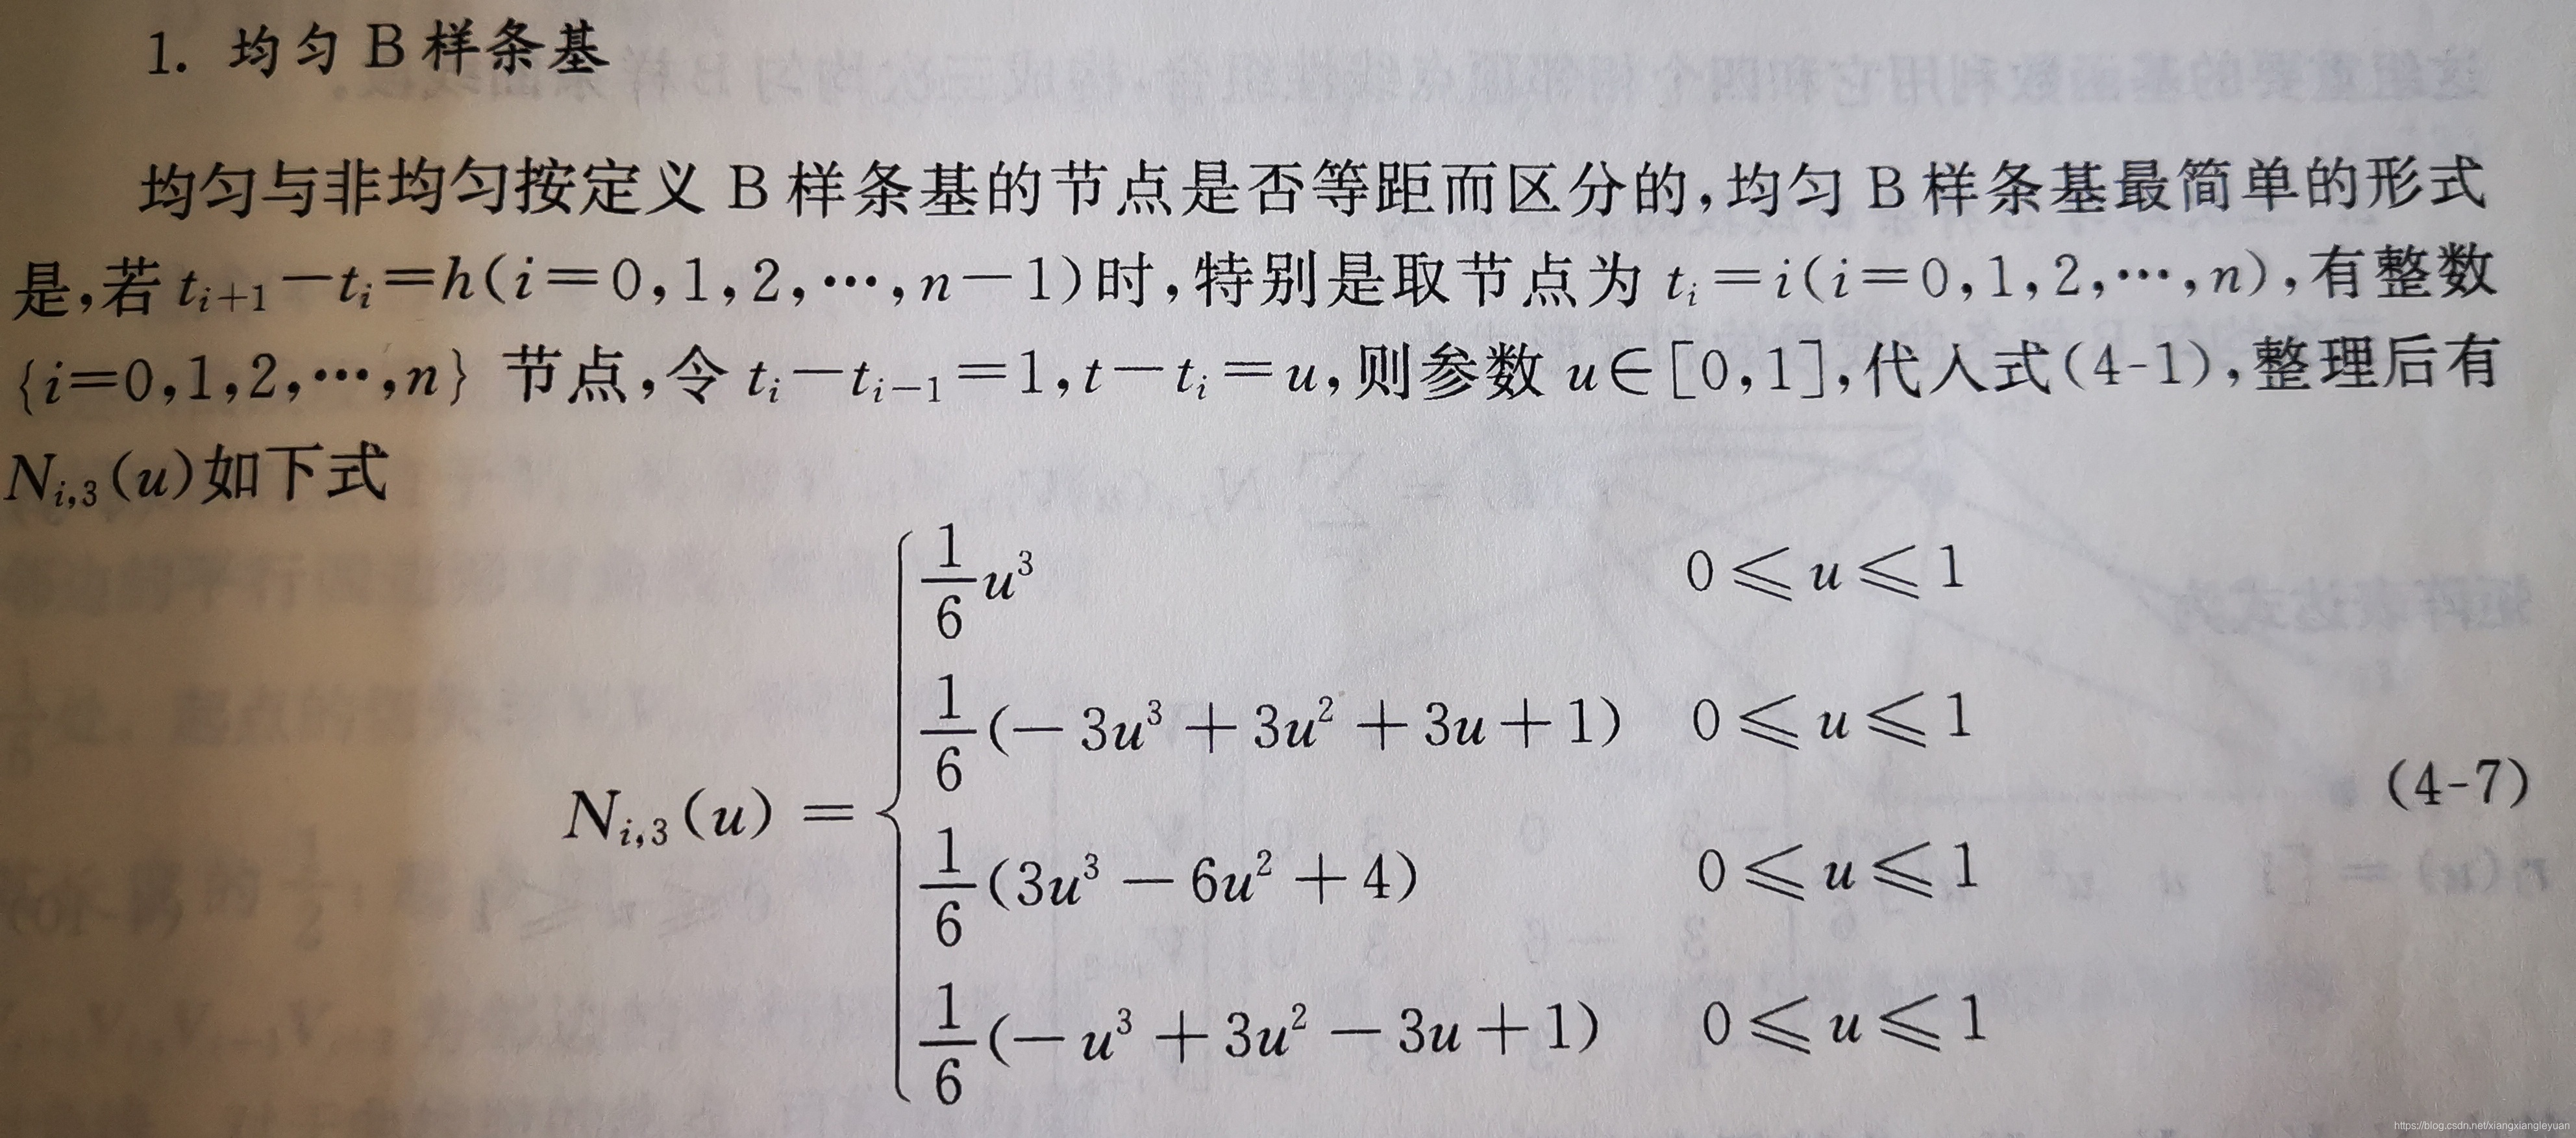
\includegraphics[scale=0.1]{./bspline-base.jpg}
\subsection{Cohen-Sutherland裁剪算法}
\paragraph{} 算法主要分三步进行:
\paragraph{1} 对线段的两个端点$P1$,$P2$编码(分别为$C1$,$C2$)。当点在矩形窗口的上、下、右、左时,分别将第$1$、$2$、$3$、$4$位置为$1$,否则为$0$。例如,若端点在矩形内部,则编码为0000,若在左下角,则编码为0101.
\paragraph{2} 根据$C1$,$C2$尽可能多的提前判断出特殊情况,尽可能避免求交点的计算。若$C1=C2=0$,则线段完全在窗口内,保留整条线段。若$C1\land C2\ne 0$,说明两端点在矩形的同侧,也就是整个在矩形外部,整个丢弃。若为其他情况,则进入第三步。
\paragraph{3} 根据$P1$的编码值,确定其在哪条边界线之外,求线段与该边界线的交点$P$,交点把线段分成两段,舍去$P1P$段,把交点$P$作为剩余线段的$P1$端点重新进行第二步。
\subsection{Liang-Barsky}

\paragraph{}Liang-Barsky从直线的参数方程角度出发,直接求出直线在窗口内的部分。考虑直线的参数方程:\\
$$x=x_0+t(x_1-x_0)=x_0+t\Delta x,$$
$$y=y_0+t(y_1-y_0)=x_0+t\Delta y$$
其中$t\in [0,1]$
\paragraph{}如果线段上一点$P(x,y)$位于坐标$(x_{min},y_{min})$和$(x_{max},y_{max})$确定的窗口内,则有下列不等式成立:\\
$$x_{min}\le x_0+t\Delta x\le x_{max}$$
$$y_{min}\le y_0+t\Delta y\le y_{max}$$
\paragraph{}这四个不等式可以表示为:
$$tp_i\le q_i, i=1,2,3,4(\star)$$
其中,\\
$$p_1=-\Delta x,q_1=x_0-x_{min}$$
$$p_2=\Delta x,q_2=x_{max}-x_{0}$$
$$p_3=-\Delta y,q_3=y_0-y_{min}$$
$$p_4=\Delta y,q_4=y_{max}-y_{0}$$
\paragraph{} 根据$\star$式,\\
\paragraph{1} 若对于某个$i$,$p_i=0$,即直线与窗口的某一条边平行,若$q_i<0$,则第$i$个不等式恒不成立,说明线段全部在裁剪窗口外,整个舍去。
\paragraph{2} 否则,可以直接求解$\star$式。若$p_i<0$,线段从裁剪边界延长线的外部延伸到内部;若$p_i>0$,线段从裁剪边界延长线的内部延伸到外部。然后求出$t$的上下界$u_1$和$u_2$。初始时,$u_1=0,u_2=1$。若$p_i<0,u_1=\max(u_1,\frac{q_i}{p_i})$;若$p_i>0,u_2=\min(u_2,\frac{q_i}{p_i})$。若$u_1>u_2$,说明线段全部在裁剪窗口外,整个舍去;否则,根据$t$的取值范围算出$x,y$的取值集合。(维基百科)
\section{系统介绍}
\subsection{命令行程序}
cg\_cli.py是输入处理程序,从input逐行读入并解析指令。当遇到"drawxxxx"时,将指令封装成$item\_dict$中的一个条目,然后在图片保存时,通过调用cg\_algorithms.py中的算法将其绘制在canvas(画布)上;当遇到"rotate","scale","clip"时,直接从$item\_dict$中查找对应的条目并调用algorithm模块对该条目中的属性进行修改,达到放缩、旋转、裁剪图形的效果。

\subsection{图形界面程序}
\paragraph{}我直接在助教写的框架基础上扩展。框架的交互逻辑大致如下:
\paragraph{}首先,main函数调用了MainWindow构造函数,MainWindow类继承了QMainWindow类,创建并初始化了图元选择表(使用QListWidget类)、画布(使用MyCanvas类,该类也需要自己实现)和菜单栏(使用menuBar成员函数)。然后需要设置主窗口的布局,我按照默认框架使用了水平布局,先按顺序将画布和图元选择表加入布局hbox\_layout,然后将主窗口的布局设置为hbox\_layout,即可实现从左到右依次为画布和图元选择表的效果。为了实现鼠标点击使用菜单栏的效果,需要为菜单栏加入功能组件,然后为每个组件编写一个槽函数,并将两者进行信号连接。
\paragraph{}如上文所提到的,MyCanvas类继承自QGraphicsView类,是自定义的画布类,该类中,除去一些必要的画图/编辑操作前后的函数(设置选择图元编号、设置当前画图状态、算法等),最重要的就是重写鼠标的点击/移动/松开事件,以实现鼠标操纵画图/对图元编辑的效果。对于不同的画图操作,它们的共同点是,首先通过MyItem类创建一个item,添加到成员变量scene中(scene由QGraphicsScene类创建,用来记录画布中的图元信息),然后通过鼠标所在的位置,计算必要的参数(cg\_algorithms中的算法所需要的)。对于旋转裁剪等编辑操作,则需要通过选择的编号找出对应的item,计算必要的参数,根据对应的算法函数修改item。
\paragraph{}MyItem类继承自QGraphicsItem类,用于定义一个图元,根据文档规定,需要重写boundingRect(用矩形定义图元的外部边界)和paint函数(逐个像素点绘制即可),然后在MyCanvas类的成员函数中调用updateScene时会将图元绘制到画布上。
\section{总结}
通过本次图形学大作业,我对课程所学的算法使用代码自己实现了一遍,加深了理解;另外,我还学习了pyqt5框架的使用,收获很大。
\section{参考资料}
\paragraph{} 包括学习算法所用的资料和编写gui界面所需的资料\\
\url{https://en.wikipedia.org/wiki/Digital_differential_analyzer_(graphics_algorithm)}\\
\url{https://en.wikipedia.org/wiki/Bresenham\%27s_line_algorithm}\\
\url{https://blog.csdn.net/qq_42185999/article/details/102377383}\\
\url{https://en.wikipedia.org/wiki/B\%C3\%A9zier_curve}\\
\url{https://zhuanlan.zhihu.com/p/144042470}\\
\url{https://en.wikipedia.org/wiki/Cohen\%E2\%80\%93Sutherland_algorithm}\\
\url{https://en.wikipedia.org/wiki/Liang\%E2\%80\%93Barsky_algorithm}\\
\url{https://doc.qt.io/qt-5/}

\bibliographystyle{plain}%
%"xxx" should be your citing file's name.
\bibliography{xxx}

\end{document}
